% Gemini theme
% See: https://rev.cs.uchicago.edu/k4rtik/gemini-uccs
% A fork of https://github.com/anishathalye/gemini

\documentclass[final]{beamer}

% ====================
% Packages
% ====================

\usepackage[T1]{fontenc}
\usepackage{lmodern}
\usepackage[size=custom,width=121.92,height=60.96,scale=1.0]{beamerposter}
\usetheme{gemini}
% \usecolortheme{uchicago}
\usecolortheme{stanford}
\usepackage{graphicx}
\usepackage{booktabs}
\usepackage{tikz}
\usepackage{pgfplots}
\usepackage[most]{tcolorbox}
\usepackage[export]{adjustbox}
\pgfplotsset{compat=1.17}

\definecolor{mycolor}{RGB}{173,10,29}

\AtBeginDocument{
  \fontsize{32pt}{0.5ex} % Adjust 12pt to your desired font size, and 14pt to a suitable line spacing
}

% ====================
% Lengths
% ====================

% If you have N columns, choose \sepwidth and \colwidth such that
% (N+1)*\sepwidth + N*\colwidth = \paperwidth
\newlength{\sepwidth}
\newlength{\colwidth}
\newlength{\widecolwidth}
\setlength{\sepwidth}{0.0001\paperwidth}
\setlength{\colwidth}{50cm}
\setlength{\widecolwidth}{60cm}

\title{From Possible to Pause-able:\linebreak Children's hesitancy may mark implicit skepticism of incorrect intuitive beliefs}

\author{Adani Abutto\inst{a, b} \and Igor Bascandziev\inst{a} \and Caren Walker\inst{c} \and Elizabeth Bonawitz\inst{a}}

\institute[shortinst]{\inst{a} Harvard University \samelineand \inst{b} Stanford University \samelineand \inst{c} University of California San Diego}

% ====================
% Footer (optional)
% ====================

\footercontent{
  \hspace{8ex}We thank families for their participation, and the Caplan Foundation, James S. McDonnell Foundation, and Jacobs Foundation for their generous support of this research. \hfill
  Contact: \href{mailto:aabutto@stanford.edu}{aabutto@stanford.edu}  || \href{https://adaniabutto.com}{stanford.edu/$\sim$aabutto}\hspace{8ex}}

% ====================
% Logo (optional)
% ====================

% use this to include logos on the left and/or right side of the header:
 \logoright{
\includegraphics[height=7.5cm]{stanford_logos/hgse_logo_clear.png}}
 \logoleft{
\includegraphics[height=7.5cm]{stanford_logos/CoCoDev_Logo.png}}

% ====================
% Body
% ====================

\begin{document}

\begin{frame}[t]
\begin{columns}[t]

\begin{column}{\colwidth}

  \begin{block}{BACKGROUND}

    \begin{itemize}
          \item \emph{"Air is nothing!"} Young children’s naive, \textbf{intuitive beliefs} about the material world are theory-like but \textbf{often run counter to scientific understanding}\textsuperscript{[1, 2]}
      \item Between ages 6-12, in an episode of conceptual change, children start revising their "theory of matter"\textsuperscript{[1]}
      \item \textbf{Even \emph{before}} acquiring beliefs aligned with \textbf{scientific understanding}, learners'  \textbf{other knowledge can be inconsistent with naive beliefs} (e.g., \emph{"we need air to breathe"})
       \item This belief inconsistency may lead to slower answers to ”incongruent” questions (naive answer ≠ correct answer; typically undergoing change) than ”congruent” questions (naive answer = correct answer)
    \end{itemize}
    
	\begin{tcolorbox}[
		colback=mycolor,
		colframe=mycolor,
		coltext=white,
		boxsep=4pt,
		left=2mm,
		right=2mm,
		top=2mm,
		bottom=2mm,
		arc=5mm,
		auto outer arc,
		boxrule=4pt,
		width=\dimexpr\linewidth-2\fboxsep\relax,
		]
		\centering
		\textbf{Do children at the brink of revising their naive beliefs about the material world show slower response times for "theory-incongruent" questions than "theory-congruent" questions?}
	\end{tcolorbox}


  \end{block}

  \begin{block}{PROCEDURE}
  
  \centering Children answered 36 forced-choice questions about 10 entities and their physical properties\newline(e.g., cats, rocks, shadows; air, steam, electricity)
    
    \begin{figure}
      \centering
	{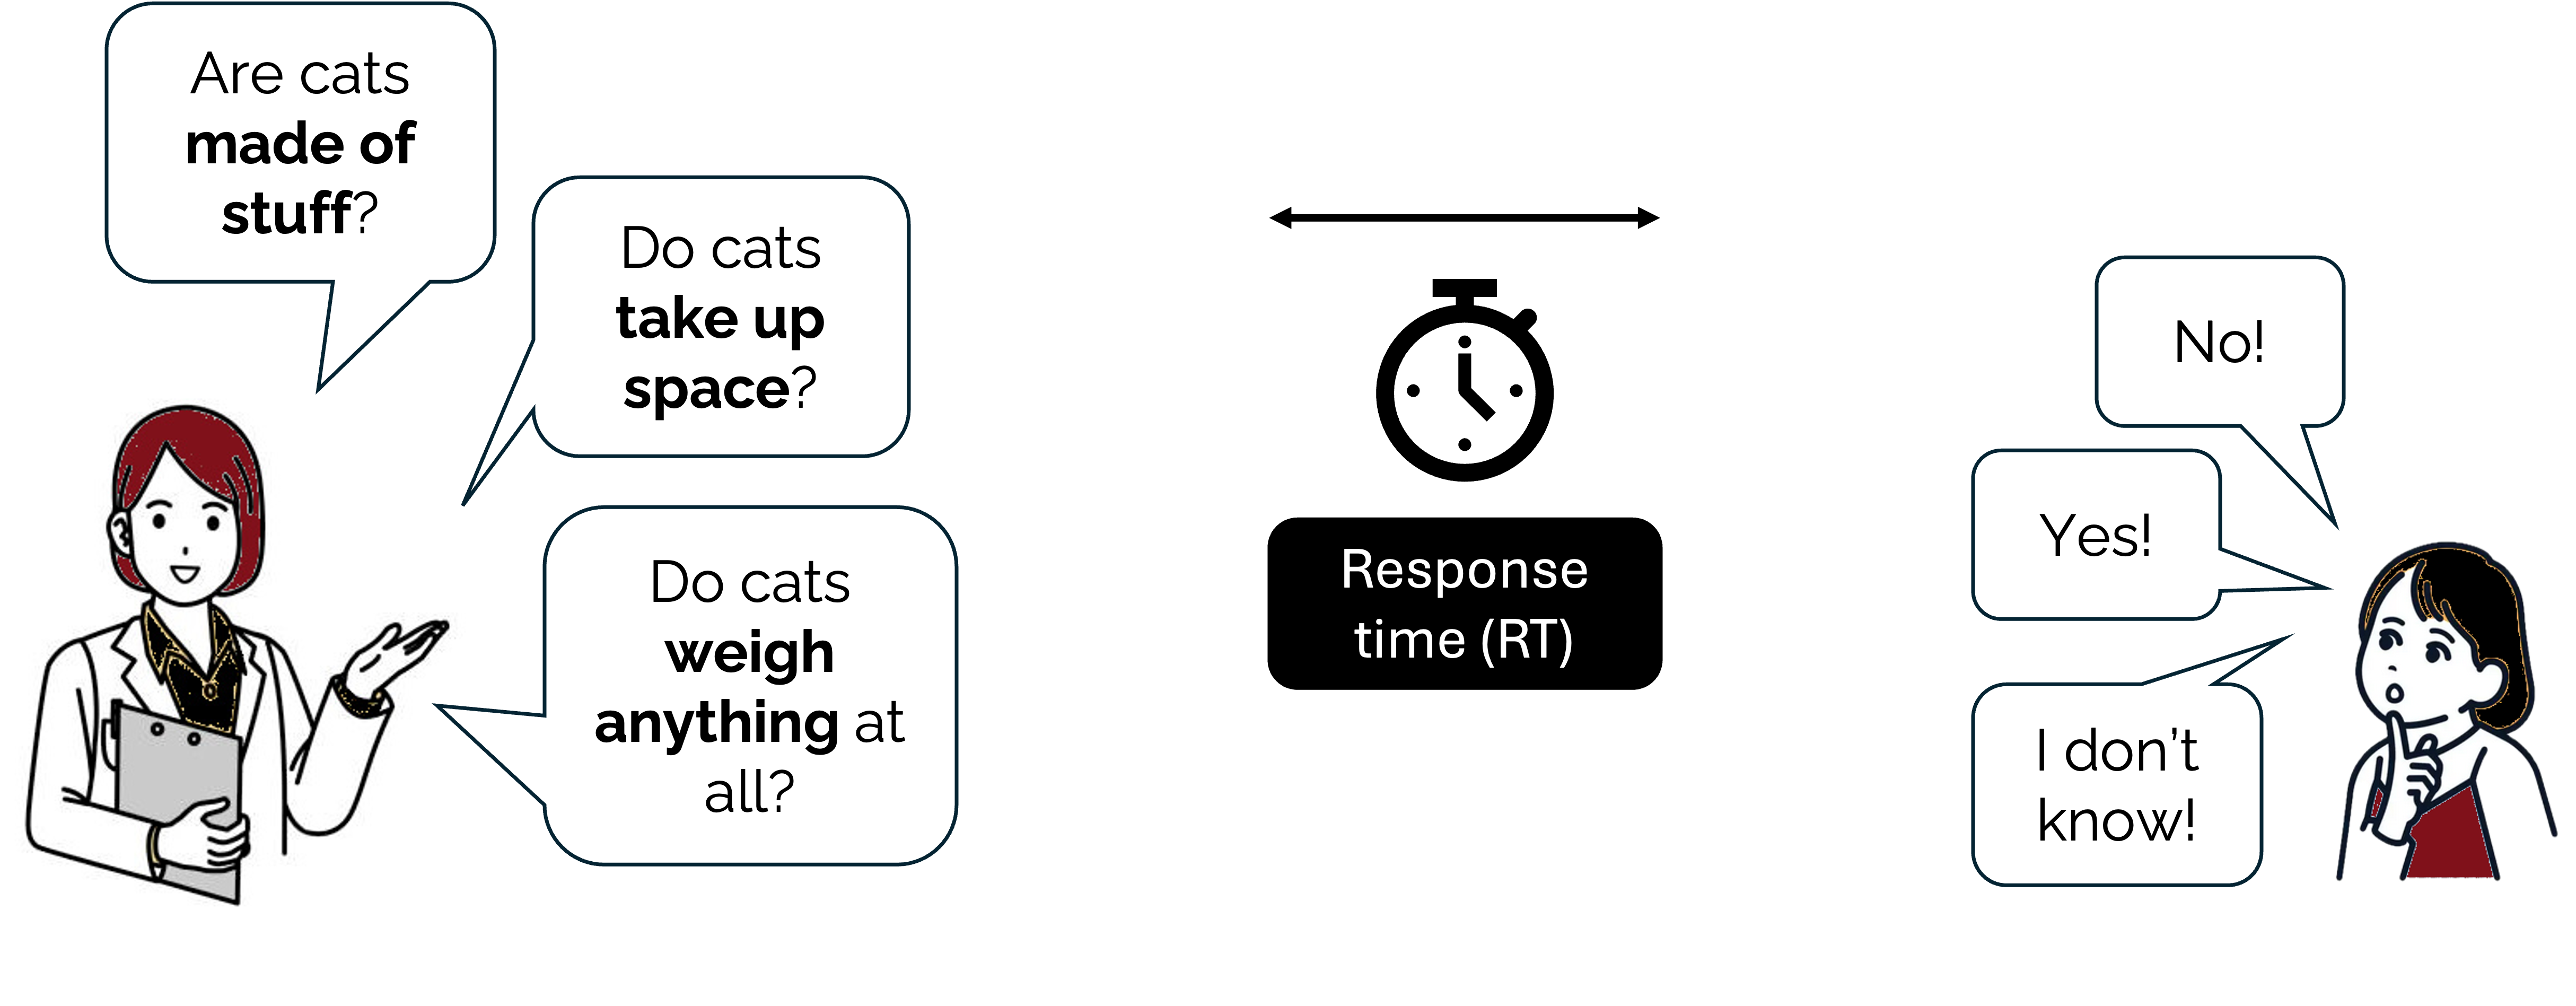
\includegraphics[height=14cm]{images/procedure6.png}}\\[-1ex]
    \end{figure}

    \begin{itemize}
	\item Based on \textbf{video}, we \textbf{coded children's RTs} (time between end of question and start of response)
	\item Selected subset: \textbf{Congruent} questions (k = 5) were those \textbf{most children answered correctly}; \textbf{incongruent} questions (k = 5) were those \textbf{fewest children answered correctly}
	\item We excluded children's RTs for inaccurate (congruent q.) and accurate (incongruent q.) responses
    \end{itemize}
    
  \end{block}

\end{column}

\begin{column}{\widecolwidth}

  \begin{block}{RESULTS}

\begin{minipage}{0.55\textwidth}
\centering
    \begin{figure}
      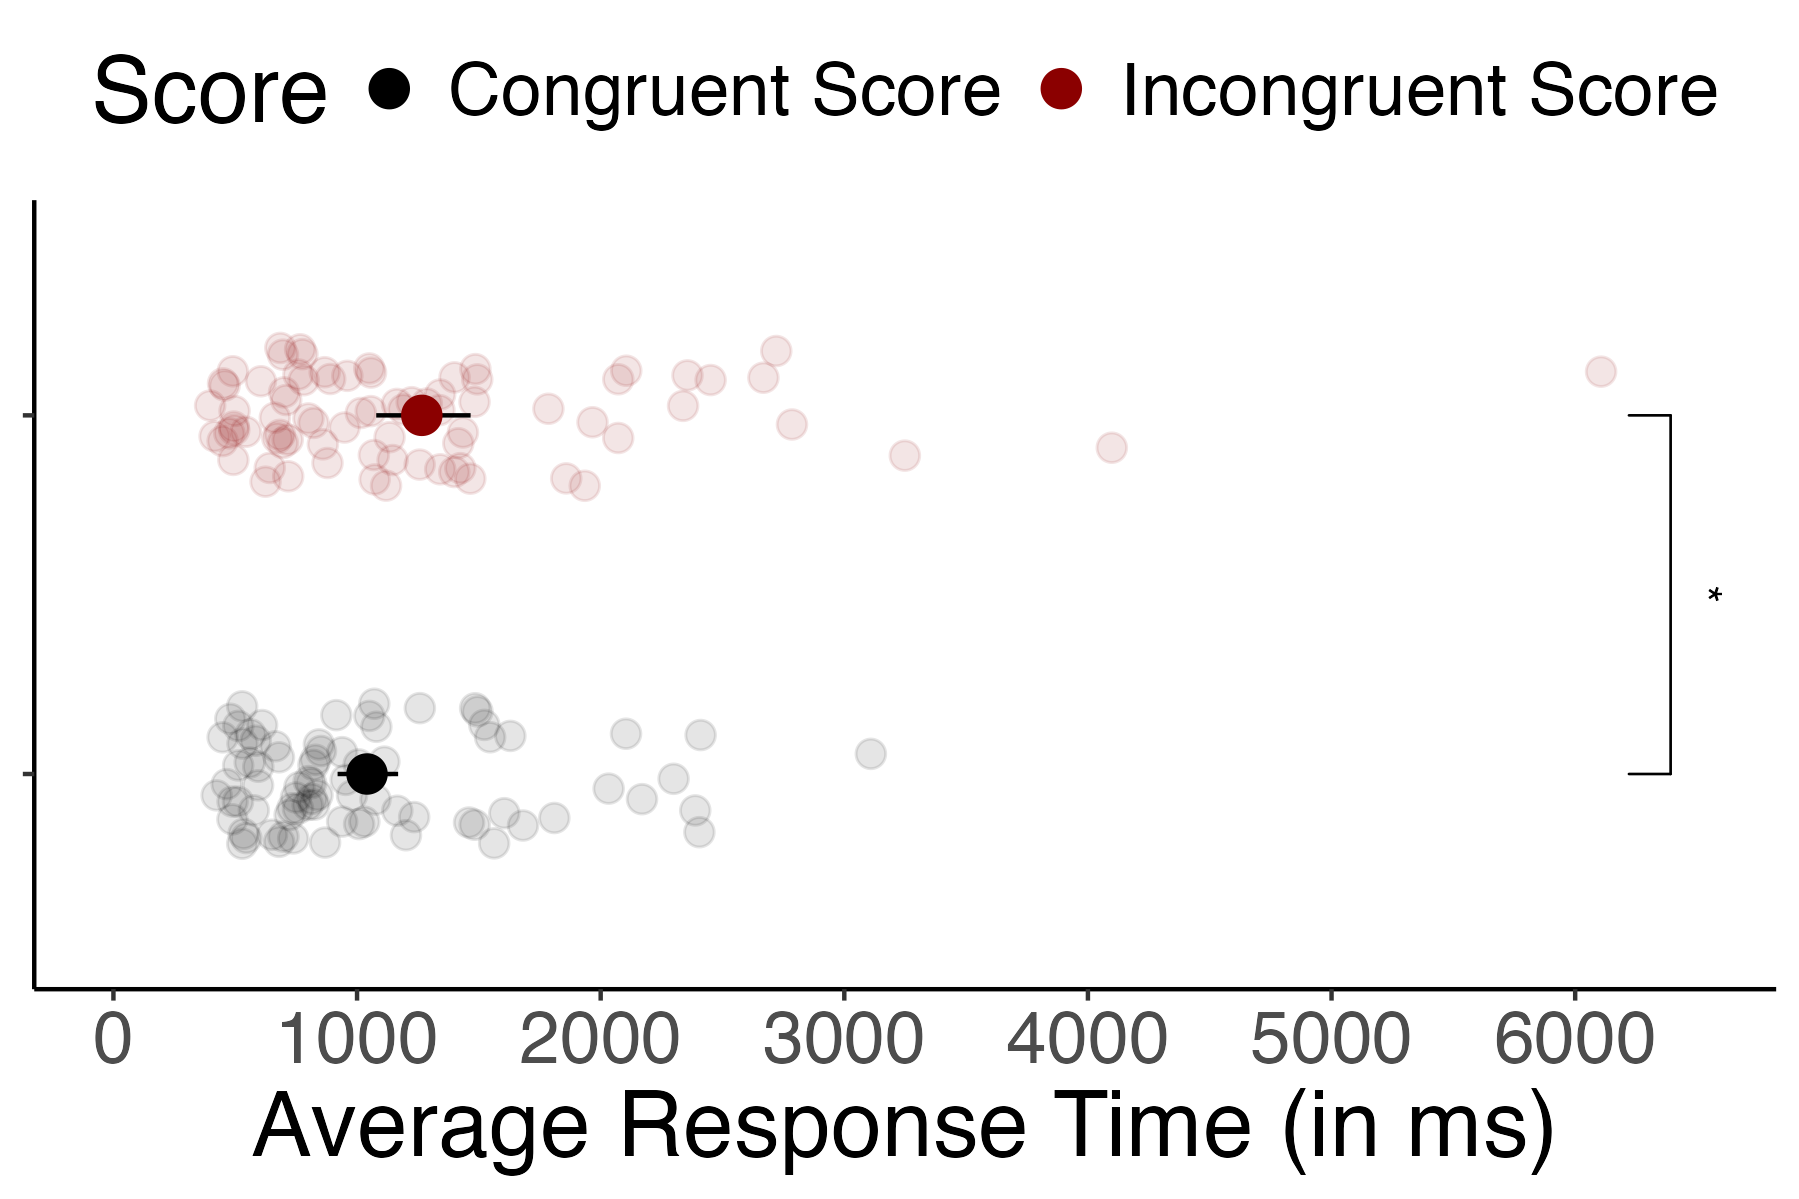
\includegraphics[height=19cm]{plots/figure1.png}
    \end{figure}
{\footnotesize Error bars are bootstrapped 95\% CIs. Second coder coded 100\% of RT data; ICC = .84 (congruent); .95 (incongruent).}
\end{minipage}%
\begin{minipage}{0.45\textwidth}
\begin{figure}
      \centering
      \href{https://aspredicted.org/DJG_YWR}{
\includegraphics[height=2.125cm]{images/osf.png}}
      \href{https://aspredicted.org/DJG_YWR}{
\includegraphics[height=2.5cm]{images/aspredicted.png}}\\[2ex]
\end{figure}
\center{\Large\textbf{\emph{N} = 79 five- to nine-year-old children} (\emph{M} = 7.4 yrs)}\\[2ex]
    \begin{itemize}
        \item Overall, children were \textbf{marginally slower answering \emph{incongruent} questions} (\emph{d}  = 0.24, \emph{p} = .041)
        \item Children \textbf{varied considerably} in their incongruent-congruent difference ("difference score")
        \item Difference score \textbf{correlated moderately with EFs} and \textbf{domain knowledge} (\emph{r} = .28, \emph{p} = .021; \emph{r} = .31, \emph{p} = .005)
        \item No correlation between difference score and children's error monitoring or cognitive reflection abilities
    \end{itemize}
\end{minipage}
\end{block}
    
\begin{block}{DISCUSSION \& FUTURE DIRECTIONS}
	\begin{tcolorbox}[
		colback=mycolor,
		colframe=mycolor,
		coltext=white,
		boxsep=2pt,
		left=2mm,
		right=2mm,
		top=2mm,
		bottom=2mm,
		arc=5mm,
		auto outer arc,
		boxrule=4pt,
		width=\dimexpr\linewidth-2\fboxsep\relax,
		]
		\centering
		\textbf{Children's RTs may be reflective of their being at the cusp of overturning their naive beliefs about the material world}
	\end{tcolorbox}
	
    \begin{itemize}
      \item \textbf{Even before acquiring a scientific understanding} of matter and its properties, \textbf{elementary schoolers show signs of hesitancy} when producing responses invoking incorrect naive beliefs
      \item \textbf{Learners vary in their degree of hesitancy}; individual differences relate to levels of EF and overall domain knowledge
      \item We plan to replicate and extend this finding using a question set a) including items beyond the physical reasoning domain, and b), explicitly controlling for age of acquisition and processing-relevant variables (word frequency and length, no. of syllables)
    \end{itemize}
\end{block}

  \begin{block}{REFERENCES}
  \footnotesize
	[1] Carey, S. (2009). The Origin of Concepts. Oxford University Press.\\[.5ex]
	[2] Shtulman, A. (2017). Scienceblind: Why Our Intuitive Theories About the World Are So Often Wrong. Hachette UK.
  \end{block}

\end{column}
\end{columns}
\end{frame}

\end{document}
